\begin{figure}[t]
\centering
    \begin{subfigure}[t]{0.45\textwidth}
    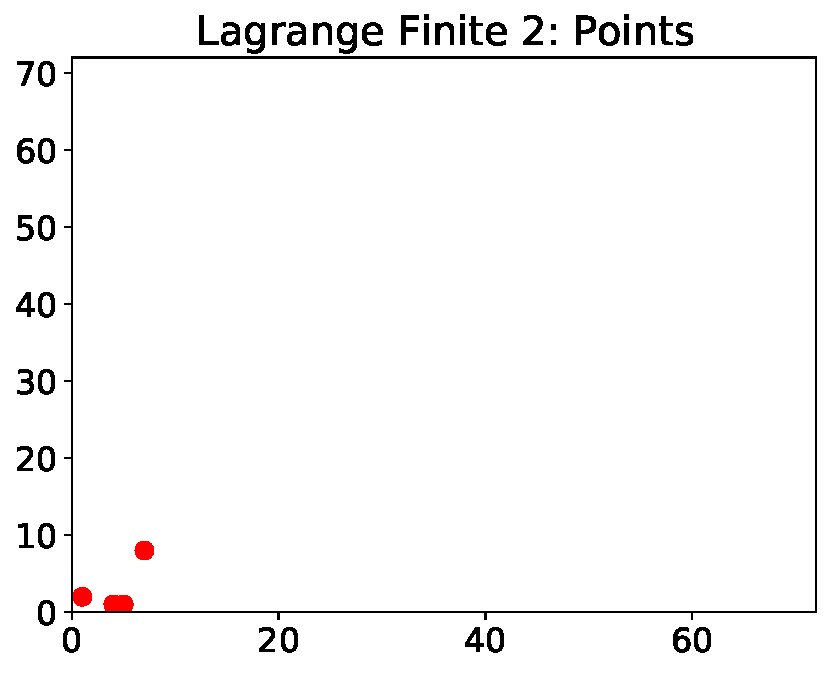
\includegraphics[width=\textwidth]{plots/lagrange/lagrange_finite_points_2.pdf}
    \caption{Lagrange interpolation data points}
    \label{fig:lagrange_finite_points_2}
    \end{subfigure}
    \begin{subfigure}[t]{0.45\textwidth}
    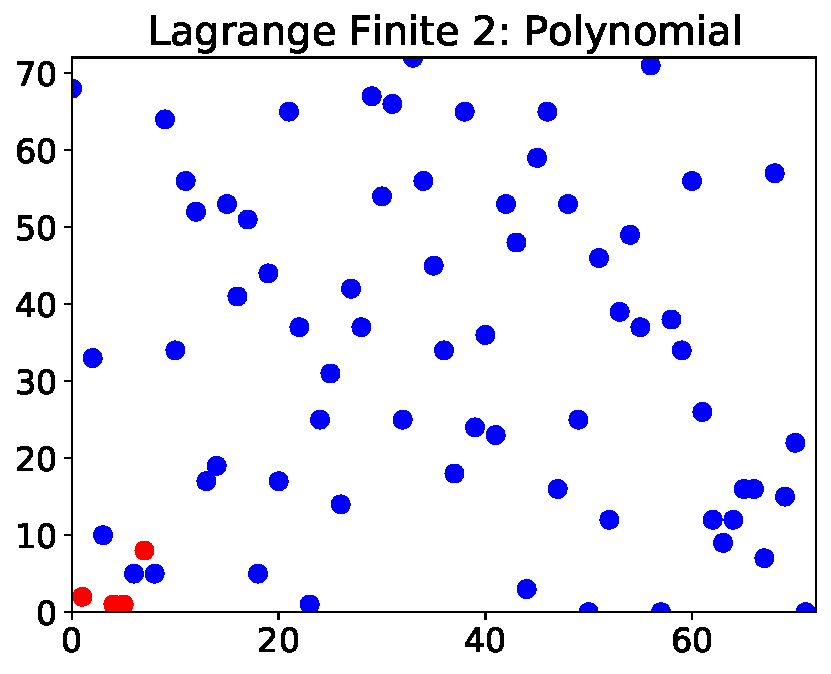
\includegraphics[width=\textwidth]{plots/lagrange/lagrange_finite_poly_2.pdf}
    \caption{Lagrange interpolation polynomial}
    \label{fig:lagrange_finite_poly_2}
    \end{subfigure}
    \caption[Data points and Lagrange Interpolation over finite fields 2]{Here
        are data points and Lagrange interpolating polynomial
        for Example~\ref{example:math_lagrange_finite_2}.
        This example uses the \gls{finite field} $\F_{73}$.}
\end{figure}

